\documentclass[12pt,fleqn]{article}\usepackage{../../common}
\begin{document}
Iki Imaj Kullanarak 3 Boyutta Tekrar Olusturmak (3D Reconstruction from Two Images)

\begin{minted}[fontsize=\footnotesize]{python}
from mpl_toolkits.mplot3d import axes3d
import scipy.linalg as lin
import cv2

dir = "/home/burak/Documents/Dropbox/Public/data/pcv_data"
img1 = cv2.imread(dir + "/alcatraz1.jpg")
img2 = cv2.imread(dir + "/alcatraz2.jpg")

detector = cv2.ORB_create( nfeatures = 10000 )

def detect_features(frame):
    keypoints, descrs = detector.detectAndCompute(frame, None)
    if descrs is None: descrs = []
    return keypoints, descrs

FLANN_INDEX_LSH    = 6
flann_params= dict(algorithm = FLANN_INDEX_LSH,
                   table_number = 6, # 12
                   key_size = 12,     # 20
                   multi_probe_level = 1) #2


kp1, des1 = detect_features(img1)
kp2, des2 = detect_features(img2)

matcher = cv2.FlannBasedMatcher(flann_params, {})
matches = matcher.knnMatch(des1, des2, k = 2)

matches = [m[0] for m in matches \
           if len(m) == 2 and m[0].distance < m[1].distance * 0.75]

print 'matches', len(matches)

pts1 = []; pts2 = []

for i in range(len(matches)):
    pt_a = kp1[matches[i].queryIdx].pt
    pt_b = kp2[matches[i].trainIdx].pt
    pt_a = np.array(pt_a).astype(int)
    pt_b = np.array(pt_b).astype(int)
    if np.sqrt(np.dot(pt_b-pt_a,pt_b-pt_a)) < 200:
        pts1.append(pt_a)
        pts2.append(pt_b)
        cv2.line(img1, tuple(pt_a), tuple(pt_b), (255, 0, 0), 5)
        cv2.circle(img1,tuple(pt_b), 5, (0,0,255), -1)

h,w,d = img1.shape
tmp = cv2.resize(img1, (int(w/4),int(h/4)))
cv2.imwrite('vision_20recons_01.jpg',tmp)

for pt in pts2: cv2.circle(img2,tuple(pt),5,(0,0,255),-1)
tmp = cv2.resize(img2, (int(w/4),int(h/4)))
cv2.imwrite('vision_20recons_02.jpg',tmp)
\end{minted}

\begin{verbatim}
matches 1277
Out[1]: 
True
\end{verbatim}

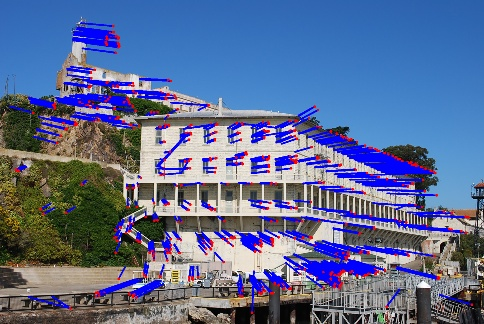
\includegraphics[width=30em]{vision_20recons_01.jpg}

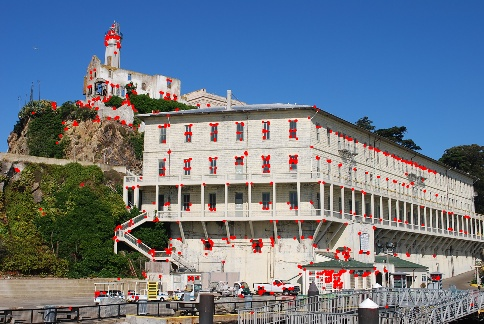
\includegraphics[width=30em]{vision_20recons_02.jpg}


\begin{minted}[fontsize=\footnotesize]{python}
# kamera matrisi biliniyor
K = np.array([[2394,0,932],[0,2398,628],[0,0,1]])
\end{minted}





















\end{document}




















